\subsection{Mолекула метана}
\lettrine[lines=3,slope=1pt,nindent=4pt]{M}{}
олекула метана представляет собой правильный тетраэдр.
Пусть одна из вершин находится в начале координат $(0,0,0)$,
одно из ребер лежит на оси $x$ и одна из граней лежит в плоскости $0yx$
и имеет длину ребра равную 1.
Определим координаты вершин для грани, лежащей в плоскости $0yx$:

\begin{tikzpicture}
\begin{scope}[xscale=6,yscale=6]
\draw(0,0) node[below left] {$0,0,0$} node[above left] {$A_1$} -- 
(1,0) node[below right] {$1,0,0$} node[above right] {$A_2$}-- 
({1/2},{sqrt(3)/2},0) node[above] 
{$A_3\;=\;{\displaystyle \frac{1}{2},\frac{\sqrt{3}}{2}},0$}
 -- (0,0);
\draw[thin,dashed] ({1/2},{sqrt(3)/2}) -- ({1/2},0) node[below] {$\frac{1}{2},0,0$};
\end{scope}
\end{tikzpicture}

из чертежа видно, что координаты векторов вершин 
$\vec{A}_1=(0,0,0)$, $\vec{A}_2=(1,0,0)$ и 
$\vec{A}_3=({\displaystyle \frac{1}{2}},{\displaystyle \frac{\sqrt{3}}{2}},0)$

координату 4-й вершины определим на проекции тетраэдра на плоскость $0yz$.

По формуле Герона площадь треугольника, если известны длины сторон, равна
$$
S = \sqrt{p(p-a)(p-b)(p-c)}, \textcyrillic{ где } p=\frac{a+b+c}{2}
$$
Отсюда найдем высоту треугольника и отношение, в котором высота делит основание:
%\begin{figure}[H]
\begin{tikzpicture}
\begin{scope}[xscale=6,yscale=6]
\draw (0,0) node [right] {$0$} --
({-sqrt(3)/2},0) node [left] {${\displaystyle \frac{\sqrt{3}}{2}}$} 
-- ({-sqrt(3)/2*1/3)}, {sqrt(2/3)}) 
node[midway,above left] {\large 1}
node[above] {$A_4$}
-- (0,0) node[midway, above right] {$\displaystyle \frac{\sqrt{3}}{2}$}
;

\draw[thin,dashed]  
({-sqrt(3)/2*1/3}, {sqrt(2/3)}) --
({-sqrt(3)/2*1/3)}, 0) node[midway, below left] {${\displaystyle \sqrt{\frac{2}{3}\;} }$};
\draw[brace,decoration={raise=2ex}] ({-sqrt(3)/2*1/3)+0.01}, 0) -- (0,0) node[midway,below,yshift=-3ex] {${\displaystyle \frac{1}{3}\frac{\sqrt{3}}{2}}$};
\draw[brace,decoration={raise=2ex}] ({-sqrt(3)/2},0) -- ({-sqrt(3)/2*1/3)-0.01}, 0) node[midway,below,yshift=-3ex] {${\displaystyle \frac{2}{3}\frac{\sqrt{3}}{2}}$};
\end{scope}
%\caption{проекция тетраэдра на ось $0yz$.}
\label{chart2}
\end{tikzpicture}
%\end{figure}

Из чертежа %(\ref{chart2}) 
видно, что координаты вершины $A_4$ равны
$$
\vec{A}_4 = \left({\displaystyle \frac{1}{2}}, {\displaystyle \frac{1}{2\sqrt{3}} }, {\displaystyle \sqrt{\frac{2}{3}}}\right)
$$

вектора вершин в координатной форме
$$ 
\vec{A}_1=\left(\begin{array}{c}0\\0\\0\\1\end{array}\right), 
\vec{A}_2 =\left(\begin{array}{c}1\\0\\0\\1\end{array}\right),
\vec{A}_3 =\left(\begin{array}{c}{\displaystyle \frac{1}{2}}\\ \\
{\displaystyle \frac{\sqrt{3}}{2}}\\ \\0\\ \\1\end{array}\right),
\vec{A}_4 =\left(\begin{array}{c}{\displaystyle \frac{1}{2}}\\ \\
{\displaystyle \frac{1}{2\sqrt{3}}}\\ \\
{\displaystyle \sqrt{\frac{2}{3}}}\\ \\1\end{array}\right).
$$ 

Координата точки, где находится атом $C$ лежит в центре тяжести:

$$
\vec{A}_5 = \frac{1}{4}
\left(\vec{A}_1 + \vec{A}_2 + \vec{A}_3 + \vec{A}_4\right)
$$

поворот вокруг оси $z$ на угол $\alpha$ представляется матрицей

$$
\mathds{A} = \left(\begin{array}{cccc}
\cos{\alpha}&-\sin{\alpha}&0&0\\
\sin{\alpha}&\cos{\alpha}&0&0\\
0&0&1&0\\
0&0&0&1
\end{array}\right)
$$

поворот вокруг оси $y$ на угол $\beta$ представляется матрицей

$$
\mathds{B} = \left(\begin{array}{cccc}
\cos{\beta}&0&-\sin{\beta}&0\\
0&1&0&0\\
\sin{\beta}&0&\cos{\beta}&0\\
0&0&0&1
\end{array}\right) 
$$

Координаты вектора  $A_i$ в результате двух поворотов будут равны
$$
\vec{A}_{i\textcyrillic{ после поворота}} = \mathds{B}\cdot \mathds{A}
\cdot \vec{A}_i
$$

Чтобы получить проекцию на плоскость $0xz$ молекулы можно
убрать $y$-координату или воспользоваться 
умножением слева на матрицу-проектор:
%http://www.latex-community.org/forum/viewtopic.php?f=5&t=2238
$$
%\mathbb{Pr}=
\mathds{P}\bf{r}=
\left(\begin{array}{cccc}1&0&0&0\\0&0&0&0\\0&0&1&0\\0&0&0&1\end{array}\right)
$$

$$
\left.\vec{A}_{i\textcyrillic{ после поворота}}\right|_{0xz} = 
\mathds{P}\bf{r}\cdot\mathds{B}\cdot \mathds{A}
\cdot \vec{A}_i
$$

Матрица-проектор имеет $det(\mathds{P}\bf{r})=0$, и значит
отображает пространство на плоскость.

 
Проекция на плоскость $0xz$ молекулы метана 
после двух последовательных поворотов
на угол ${\displaystyle \alpha=\frac{\pi}{3}}$, а затем 
на угол ${\displaystyle \beta=\frac{\pi}{6}}$ 
приведена на рисунке:

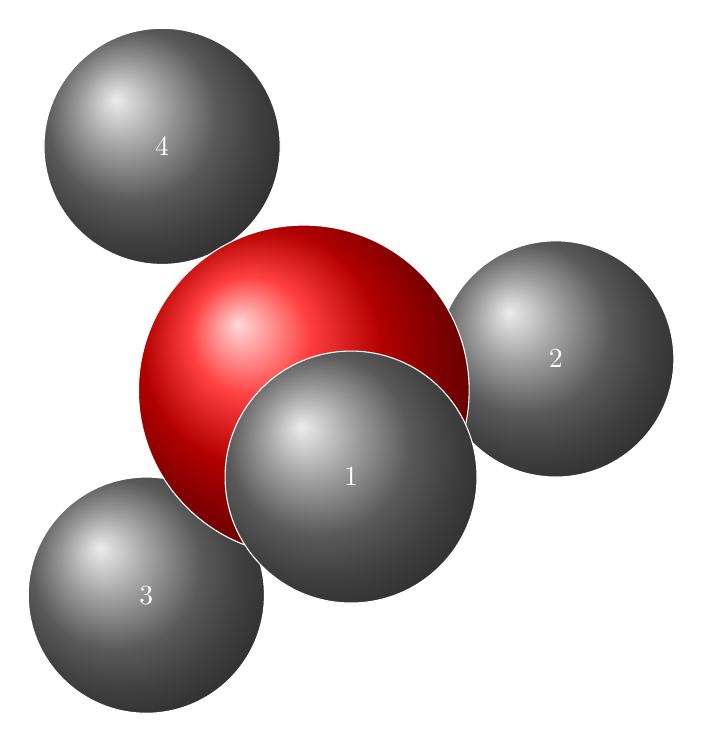
\begin{tikzpicture}
%\begin{scope}[xshift=-1cm,yshift=-5.5cm]
\draw [rounded corners=4pt,color=white,ball color=gray,smooth] (2.6,1.5) circle (1.5) node {2}; %2 
\draw [rounded corners=4pt,color=white,ball color=gray,smooth] (-2.6,-1.5) circle (1.5) node {3}; %3
%\draw [rounded corners=4pt,color=white,ball color=gray,smooth] (-2.8,3.7) circle (1.5) node {4}; %4 
\draw [rounded corners=4pt,color=white,ball color=gray,smooth] (-2.4,4.2) circle (1.5) node {4};%4
%\draw [rounded corners=4pt,color=white,ball color=red,smooth] (-0.7,0.9) circle (2.1);
\draw [rounded corners=4pt,color=white,ball color=red,smooth] (-0.6,1.1) circle (2.1);
\draw [rounded corners=4pt,color=white,ball color=gray,smooth] (0,0) circle (1.6) node {1}; %1
%\end{scope}
\end{tikzpicture}

чтобы вычислить координаты при повороте можно воспользоваться 
программой scilab:
\begin{verbatim}
a1=[0;0;0;0];
a2=[1;0;0;0];
a3=[0.5;sqrt(3)/2;0;0];
a4=[0.5;1/2/sqrt(3);sqrt(2/3);0];

alpha=%pi/3;
A=[cos(alpha),-sin(alpha),0,0;sin(alpha),cos(alpha),0,0;0,0,1,0;0,0,0,1];
beta=%pi/6;
B=[cos(beta),0,-sin(beta),0;0,1,0,0;sin(beta),0,cos(beta),0;0,0,0,1];

h1=6*B*A*a1
h2=6*B*A*a2
h3=6*B*A*a3
h4=6*B*A*a4
c=1/4*6*B*A*(a1+a2+a3+a4)
\end{verbatim}


при повороте на угол ${\displaystyle \alpha=-\frac{\pi}{3}}$, а затем
на угол ${\displaystyle \beta=-\frac{\pi}{6}}$

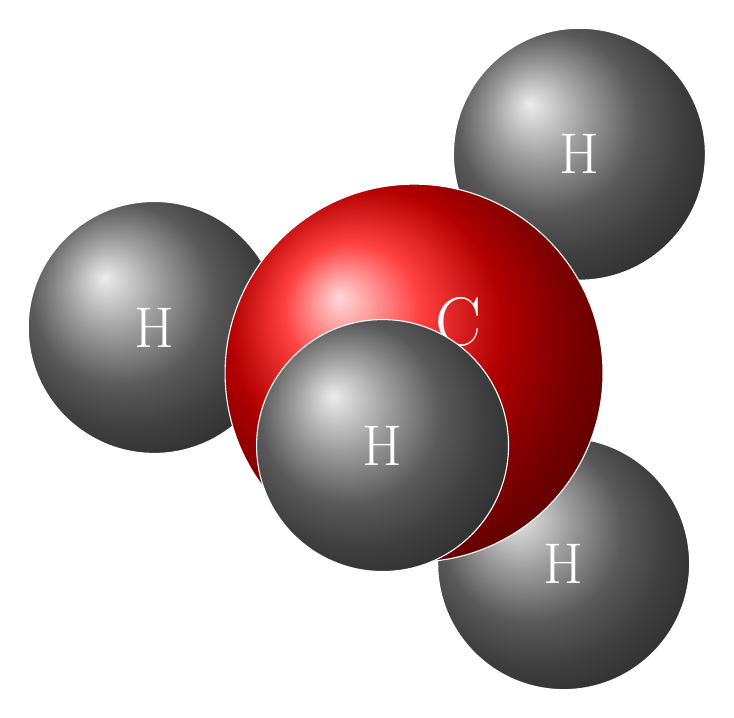
\begin{tikzpicture}
%\begin{scope}[xshift=-1cm,yshift=-5.5cm]
\draw [rounded corners=4pt,color=white,ball color=gray,smooth] (5.2,-3) circle (1.6) node {\huge H}; %3
\draw [rounded corners=4pt,color=white,ball color=gray,smooth] (5.4,2.2) circle (1.6) node {\huge H}; %4 
\draw [rounded corners=4pt,color=white,ball color=gray,smooth] (0,0) circle (1.6) node {\huge H}; %1
\draw [rounded corners=4pt,color=white,ball color=red,smooth] (3.3,-0.58) circle (2.4) 
(3.45,-0.35) node[above right] {\Huge C};
\draw [rounded corners=4pt,color=white,ball color=gray,smooth] (2.9,-1.5) circle (1.6) node {\huge H}; %2 
%\end{scope}
\end{tikzpicture}

Пример рисования в {\TeX}  шара  диаметром $1.6$ с центром в точке $(1,3)$ 
представлен ниже:
\begin{verbatim}
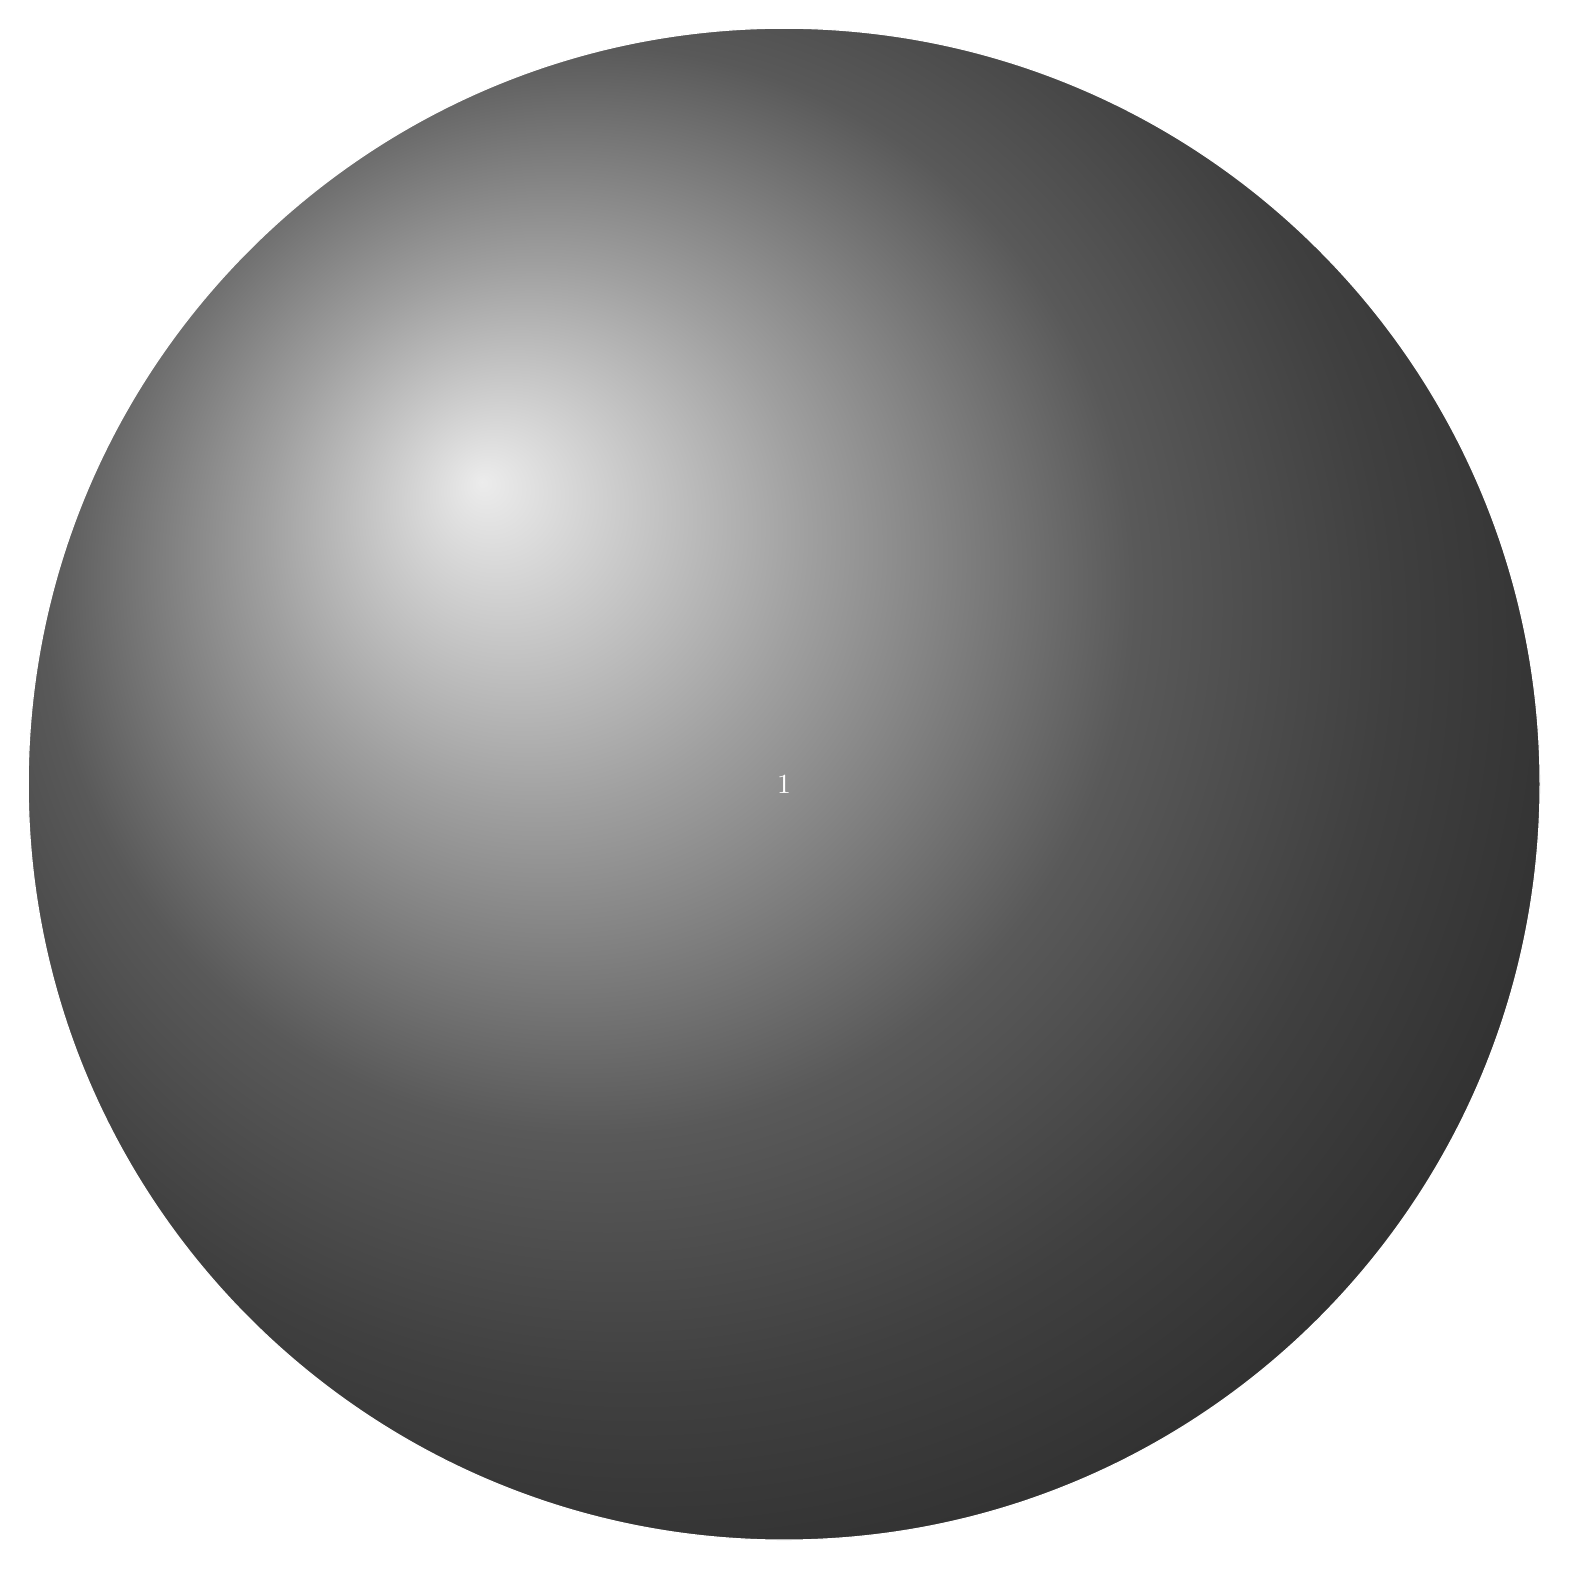
\begin{tikzpicture}
\begin{scope}[xscale=6,yscale=6]
\draw [rounded corners=4pt,color=white,ball color=gray,smooth] (1,2) 
circle (1.6) node {1}; %1
\end{scope}
\end{tikzpicture}
\end{verbatim}

\subsection{Задание практической работы №4}
\begin{tabular}{c|c|c|c}
\rotatebox{90}{\shortstack[l]{№\\варианта}}&
\rotatebox{90}{\shortstack[l]{поворот\\относительно\\оси $z$}} &
\rotatebox{90}{\shortstack[l]{поворот\\относительно\\оси $y$}} &
\rotatebox{90}{\shortstack[l]{порядок\\поворотов}}\\
\hline
&&&\\
1 & {$\displaystyle \frac{\pi}{6}$} & {$\displaystyle \frac{\pi}{6}$} & $z,y$\\
&&&\\
2 & {$\displaystyle \frac{\pi}{6}$} & {$\displaystyle \frac{\pi}{3}$} & $z,y$\\
&&&\\
3 & {$\displaystyle \frac{\pi}{6}$} & {$\displaystyle \frac{2\pi}{3}$} & $z,y$\\
&&&\\
4 & {$\displaystyle \frac{\pi}{6}$} & {$\displaystyle \frac{5\pi}{6}$} & $z,y$\\
&&&\\
5 & {$\displaystyle \frac{\pi}{3}$} & {$\displaystyle \frac{\pi}{6}$} & $z,y$\\
&&&\\
6 & {$\displaystyle \frac{\pi}{3}$} & {$\displaystyle \frac{\pi}{3}$} & $z,y$\\
&&&\\
7 & {$\displaystyle \frac{\pi}{3}$} & {$\displaystyle \frac{2\pi}{3}$} & $z,y$\\
&&&\\
8 & {$\displaystyle \frac{\pi}{3}$} & {$\displaystyle \frac{5\pi}{6}$} & $z,y$\\
&&&\\
9 & {$\displaystyle \frac{2\pi}{3}$} & {$\displaystyle \frac{\pi}{6}$} & $z,y$\\
&&&\\
10 & {$\displaystyle \frac{2\pi}{3}$} & {$\displaystyle \frac{\pi}{3}$} & $z,y$\\
&&&\\
11 & {$\displaystyle \frac{2\pi}{3}$} & {$\displaystyle \frac{2\pi}{3}$} & $z,y$\\
&&&\\
12 & {$\displaystyle \frac{2\pi}{3}$} & {$\displaystyle \frac{5\pi}{6}$} & $z,y$\\
&&&\\
\hline
\end{tabular}
 
\vskip 1cm
 
{\bf Задание:} Построить в {\TeX}  молекулу метана с заданными углами поворота 


